\chapter{CodeMarkBench Benchmark Foundation}\label{cpt:codemarkbench}

CodeMarkBench is the empirical foundation of this dissertation. Its role is not to prove that watermarking is impossible, but to create a reproducible setting in which source-code watermarking methods are evaluated under executable, multi-model, multi-language, and stress-test conditions. The benchmark is release-backed: the submitted artifact and public repository record the canonical single-host matrix with 140/140 run-completion records, four pinned runtime baselines, five local code models, and seven executed source groups~\cite{zhang2026codemarkbench}. This 140/140 figure is a reproducibility and inventory-completion result, not a watermark detection success rate.

\section{Benchmark Design}

It is useful to start from a single benchmark row. Suppose KGW is evaluated on DeepSeek-Coder for the HumanEval+ source group under identifier renaming. The generated program must first be admitted as executable code. The attacked version must also parse and pass the corresponding tests before it contributes to the robustness denominator. The detector output is then recorded together with the method version, model revision, source group, attack identity, and control status. If the same attack is applied to a clean unwatermarked solution, the detector result belongs to the negative-control denominator rather than the positive robustness denominator. This row-level discipline is what prevents the benchmark from reporting an impressive detector rate on artifacts that are not comparable.

The benchmark can be described as a tuple
\begin{equation}
  \mathcal{B} = (\mathcal{T}, \mathcal{S}, \mathcal{M}, \mathcal{W}, \mathcal{A}, \mathcal{E}),
  \label{eq:benchmark-tuple}
\end{equation}
where $\mathcal{T}$ is the set of executable task instances, $\mathcal{S}$ is the set of source groups used to construct those tasks, $\mathcal{M}$ is the model set, $\mathcal{W}$ is the watermark baseline set, $\mathcal{A}$ is the set of attacks or transformations, and $\mathcal{E}$ is the executable evaluation harness. For model $m \in \mathcal{M}$, task instance $t \in \mathcal{T}$, and watermark method $w \in \mathcal{W}$, a generated code artifact is written as
\begin{equation}
  x = G(m,t,w).
\end{equation}
An attack or edit $a \in \mathcal{A}$ produces $x_a = A_a(x)$. The benchmark then measures whether $x$ or $x_a$ remains executable, whether the watermark detector fires, how often negative controls are falsely flagged, and how much runtime overhead is introduced.

\section{Release Contract and Reproducibility}

A release contract is necessary because benchmark results are otherwise easy to move by changing model revisions, source slices, attack implementations, or failed-run handling. CodeMarkBench therefore treats the canonical run identity as part of the evidence. The public release records the model roster, baseline identifiers, source groups, execution mode, run inventory, and summary tables. A rerun is comparable only if it preserves the same execution class and denominator. This contract is especially important for watermarking because unsupported attacks or missing controls can otherwise make a method look stronger than it is.

\section{Source Groups and Canonical Matrix}

CodeMarkBench combines public executable benchmarks and crafted benchmark families. HumanEval+ and MBPP+ follow the EvalPlus extension of HumanEval and MBPP~\cite{liu2023evalplus}. HumanEval-X provides a multilingual code-generation slice~\cite{zheng2023codegeex}. MBXP-style multilingual slices follow the same motivation as MultiPL-E-style multilingual evaluation~\cite{cassano2022multiple}. Table~\ref{tab:codemarkbench-sources} summarizes the source groups used in the current release surface.

\begin{table}[htbp]
\centering
\caption{CodeMarkBench canonical source groups.}
\label{tab:codemarkbench-sources}
\compacttable
\begin{tabular}{@{}llr@{}}
\toprule
Source group & Role & Count \\
\midrule
HumanEval+ & Public executable Python tasks & 164 \\
MBPP+ & Public executable Python tasks & 378 \\
HumanEval-X & Balanced multilingual slice & 200 \\
MBXP-5lang & Balanced multilingual slice & 200 \\
Crafted Original & Manually reviewed crafted tasks & 240 \\
Crafted Translation & Cross-language crafted tasks & 240 \\
Crafted Stress & Stress-oriented crafted tasks & 240 \\
\bottomrule
\end{tabular}
\end{table}

The active model roster contains Qwen2.5-Coder 1.5B, 7B, and 14B, StarCoder2-7B, and DeepSeek-Coder-6.7B, covering the Qwen, StarCoder, and DeepSeek code-model families~\cite{hui2024qwen25coder,bigcode2024starcoder2,guo2024deepseekcoder}. The active runtime baseline methods are STONE, SWEET, EWD, and KGW. KGW follows the green-list watermarking family introduced for LLM text watermarking~\cite{kirchenbauer2023watermark}; STONE, SWEET, and EWD are release-internal runtime baselines whose implementation provenance, adaptation assumptions, and detector boundaries are recorded in the CodeMarkBench artifact rather than treated as external peer-reviewed methods~\cite{zhang2026codemarkbench}. Under the current release contract, the full matrix completes 140/140 canonical run records with no failed run in the public result surface.

The run denominator should not be confused with the task denominator. The 140 canonical runs are
\begin{equation}
  |\mathcal{W}| \times |\mathcal{M}| \times |\mathcal{S}| = 4 \times 5 \times 7 = 140.
\end{equation}
The task set is the disjoint union $\mathcal{T}=\bigsqcup_{s\in\mathcal{S}}\mathcal{T}_s$, where $\mathcal{T}_s$ is the executable task slice for source group $s$. Each run then executes the task instances in its source group. If source group $s$ contains $n_s$ executable tasks, a method-level aggregate is computed from the multiset
\begin{equation}
  \{(w,m,s,t): w\in\mathcal{W}, m\in\mathcal{M}, s\in\mathcal{S}, t\in\mathcal{T}_s\}.
\end{equation}
Attack and control metrics then expand this base multiset with the attack or control condition $a\in\mathcal{A}_{eval}$. The 140-run inventory is therefore the release scaffold, while robustness and false-positive rates are computed over attack-expanded task rows.
This distinction matters because a successful run inventory proves that no source group was silently dropped, while a detection or utility rate still depends on the number and type of executable task instances inside each source group. The dissertation therefore treats the run inventory as a reproducibility claim and the metric tables as empirical summaries over task-level records.

The purpose of this matrix is not only to rank baseline methods. It creates the first denominator contract for the lifecycle: later provenance, audit, attribution, and triage claims inherit the rule that a result is meaningful only when its executable row, control status, and exclusion policy are fixed before interpretation.

\section{Metrics}

The benchmark separates utility, detection, robustness, stealth, efficiency, and negative controls. The utility indicator is
\begin{equation}
  U(x) =
  \begin{cases}
  1, & \text{if } x \text{ passes executable tests},\\
  0, & \text{otherwise}.
  \end{cases}
\end{equation}
Here $U$ records test-pass utility for an admitted artifact, while $V_{\mathrm{attack}}$ additionally records parse-and-test validity after an attack transformation. Robust detection under attack is estimated over attacked artifacts that remain valid under the same parse-and-test contract used by the release:
\begin{align}
  \widehat{\mathrm{RobustTPR}}(w,a)
  &= \frac{
  \sum_{x\in\mathcal{X}_w}\mathbf{1}[D_w(A_a(x))=1\wedge V_{\mathrm{attack}}(A_a(x))=1]}
  {\sum_{x\in\mathcal{X}_w}\mathbf{1}[V_{\mathrm{attack}}(A_a(x))=1]},
  \label{eq:robust-tpr}
\end{align}
where $D_w$ is the detector associated with watermark method $w$ and $\mathcal{X}_w$ is the finite released set of admitted watermarked artifacts for method $w$. This finite-release estimator is conditioned on attacked outputs that still parse and execute, so it is reported together with pass-preservation and utility rather than interpreted alone. If the denominator of an attack cell is zero, that cell is reported as not estimable rather than as 0. False-positive rate is measured on the executable unwatermarked control set $\mathcal{X}_0$:
\begin{align}
  \widehat{\mathrm{FPR}}(w,a)
  &= \frac{
  \sum_{x_0\in\mathcal{X}_0}\mathbf{1}[D_w(A_a(x_0))=1\wedge V_{\mathrm{attack}}(A_a(x_0))=1]}
  {\sum_{x_0\in\mathcal{X}_0}\mathbf{1}[V_{\mathrm{attack}}(A_a(x_0))=1]}.
\end{align}
Here $\mathcal{X}_0$ is the matched admitted unwatermarked control set. The implemented benchmark uses finite-sample estimators over released rows; additional component definitions are given in Appendix~\ref{app:reproducibility}. This keeps the main text focused on the contract: executable validity determines whether an attacked row enters a robustness denominator, and clean executable controls determine the false-positive denominator. The dissertation does not claim that the displayed rates estimate a universal distribution over all future code transformations; they summarize the fixed released matrix.
The same not-estimable convention applies to false-positive cells with zero executable control denominator.
The aggregate release scalar is used only as a summary field from the public benchmark release; the dissertation keeps component metrics visible so that robustness, utility, and false-positive behavior are not hidden behind one number. The reproducible object is the component vector
\begin{equation}
  \mathbf{q}(w) = (q_{\mathrm{core}},q_{\mathrm{robust}},q_{\mathrm{utility}},q_{\mathrm{gate}},q_{\mathrm{negFPR}},q_{\mathrm{efficiency}}),
\end{equation}
where every component is normalized so that larger values indicate better behavior. For example, a false-positive component is directionally inverted from the raw false-positive rate. If a public release reports a scalar score, the release artifact must preserve its exact weights and normalization. This dissertation uses the printed scalar descriptively and does not use it as a substitute for the underlying evidence, because two methods can have similar aggregate values while failing in different ways.

The component definitions are listed in Appendix~\ref{app:reproducibility}, Table~\ref{tab:codemarkbench-components-app}. The metric definitions also make the benchmark robust to a common reporting failure. A method should not receive credit for destroying code and then preserving a watermark on the non-executable artifact. Conversely, a method with a low false-positive rate should still report the denominator from which that rate was estimated. Zero printed false positives are therefore interpreted as ``0 observed in the released denominator,'' not as proof that the false-positive probability is mathematically zero.

\section{Attack and Control Taxonomy}

The benchmark distinguishes core edits from stress edits. Core edits include whitespace normalization, comment stripping, identifier renaming, and small noise insertion. Stress edits include control-flow flattening, block shuffling, and budgeted adaptive transformations. Negative controls include human reference solutions and clean generated code without the target watermark. A watermark method is therefore evaluated not only by whether it detects its own watermarked output, but also by whether it avoids firing on code that should not contain that watermark.

\section{Validity Principles}

The benchmark uses three validity principles to avoid overstating watermark robustness. The first principle is \emph{executable preservation}. A transformation is counted as an attack outcome only when the transformed program remains executable under the benchmark tests. Formally, an attacked artifact $x_a$ contributes to a robustness denominator only when
\begin{equation}
  V_{\mathrm{attack}}(x_a)=\mathbf{1}[U(x_a)=1 \wedge \mathrm{parse}(x_a)=1].
\end{equation}
This rule prevents a detector from receiving credit for preserving a signal in code that no longer behaves as a valid program. It also prevents a method from appearing robust simply because an attack destroyed the executable artifact.

The second principle is \emph{control symmetry}. A transformation family that is applied to watermarked code should also be applied to clean or unwatermarked controls whenever possible. Without this symmetry, a method can look clean on easy controls while failing on realistic transformed controls. CodeMarkBench therefore reports negative-control false positives under executable transformations, not only on untouched clean code. This is why a nonzero negative-control rate is treated as an important result rather than as a minor implementation detail.

The third principle is \emph{release stability}. Benchmark comparisons are meaningful only when the source groups, model revisions, watermark methods, attack scripts, and failed-run policy are fixed. A later experiment may improve or extend the benchmark, but it should be recorded as a new release surface rather than silently replacing the denominator. This principle is especially important for source-code watermarking because small implementation choices, such as whether helper functions are preserved or whether parser failures are excluded, can move detector rates substantially.

These principles make CodeMarkBench more conservative than a detector-only benchmark. The cost is that some results become less visually impressive, because methods must carry utility, robustness, and false-positive behavior at the same time. The benefit is that the benchmark exposes practical failure modes that a deployment user would actually encounter.

\section{Headline Results}

Table~\ref{tab:codemarkbench-leaderboard} reports the method-level headline surface. No evaluated baseline dominates all dimensions. SWEET and EWD have the highest descriptive release scalar in the current table, while KGW shows the highest robustness among the displayed rows. STONE has the highest gate value but also a nonzero negative-control false-positive rate. These differences support the dissertation's central motivation: source-code watermarking requires multidimensional evaluation rather than a single pass/fail detector result. They also define the downstream handoff: robustness--utility tension motivates SemCodebook, negative-control sensitivity motivates CodeDye, detector evidence without source binding motivates ProbeTrace, and missing security semantics motivates SealAudit.

\begin{table}[htbp]
\centering
\caption{CodeMarkBench headline method results. The scalar is descriptive; component metrics and denominators are primary.}
\label{tab:codemarkbench-leaderboard}
\compacttable
\begin{tabular}{@{}lrrrrrr@{}}
\toprule
\textbf{Method} & \textbf{Core} & \textbf{Robust.} & \textbf{Utility} & \textbf{Gate comp.} & \textbf{Neg. FPR} & \textbf{Scalar} \\
\midrule
SWEET & 0.5904 & 0.3361 & 0.6467 & 0.4984 & 0.0000 & 0.3827 \\
EWD & 0.5687 & 0.2645 & 0.6467 & 0.5000 & 0.0000 & 0.3761 \\
STONE & 0.5843 & 0.3536 & 0.6509 & 0.5266 & 0.1465 & 0.3504 \\
KGW & 0.5062 & 0.4439 & 0.6476 & 0.4920 & 0.0000 & 0.3498 \\
\bottomrule
\end{tabular}
\end{table}

The release inventory denominator for Table~\ref{tab:codemarkbench-leaderboard} is 140 model-method-source runs; the displayed component values are task-level aggregates inside those runs. A printed 0.0000 means no observed false positives in the released negative-control denominator, not zero false-positive risk. The table is therefore a compact release summary, not a statistical claim that every possible method, model, or attack has been exhaustively characterized.
The gate component is a normalized release metric, not a binary accept/reject decision. A high gate component does not override robustness, utility, or negative-control behavior.

\begin{figure}[htbp]
  \centering
  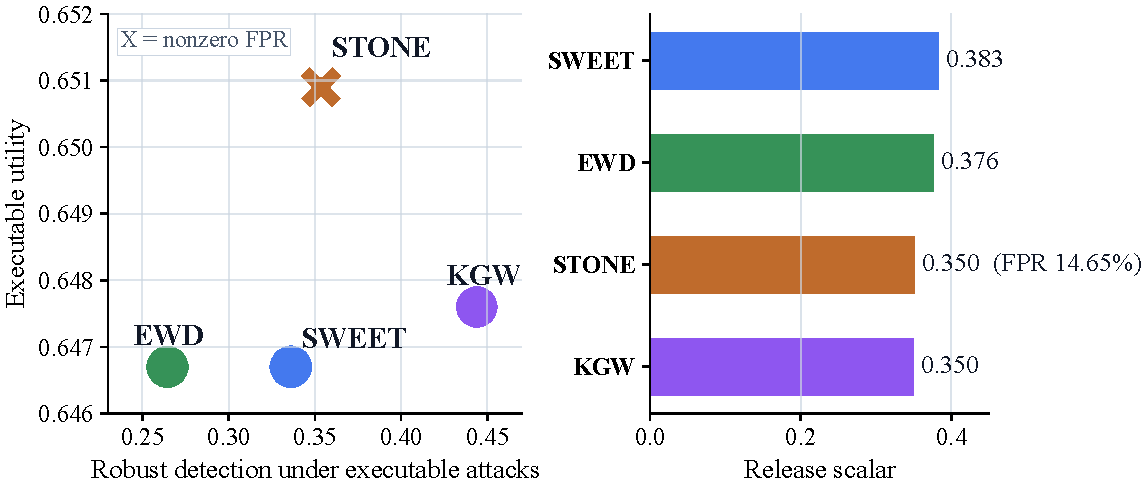
\includegraphics[width=0.96\textwidth]{fig/codemarkbench_tradeoff.pdf}
  \caption{CodeMarkBench robustness--utility tradeoff with descriptive release-scalar context. Conclusions use component coordinates and raw FPR, not a winner-takes-all ranking.}
  \label{fig:codemarkbench-tradeoff}
\end{figure}

\section{Interpretation}

The benchmark result should be read carefully. It does not imply that source-code watermarking is futile. It shows that under an executable release contract, existing runtime baselines exhibit tradeoffs across detection, robustness, utility, stealth, efficiency, and false positives. This finding motivates the rest of the dissertation. SemCodebook asks whether structured program carriers can provide stronger white-box provenance. CodeDye, ProbeTrace, and SealAudit ask how watermark evidence should be handled in black-box audit, source attribution, and safety triage settings.

More concretely, the benchmark exposes four downstream needs. Robustness and utility tradeoffs motivate SemCodebook's structured carrier design. Negative-control discipline motivates CodeDye's refusal to turn sparse black-box evidence into a prevalence claim. The fact that benchmark detection is not the same as source ownership motivates ProbeTrace's active registry. Finally, executable benchmarks still do not answer whether watermark mechanisms can interact with unsafe code behavior, which motivates SealAudit. CodeMarkBench is therefore not just an opening experiment; it supplies the problem decomposition used by the rest of the thesis.

The benchmark also clarifies how to read zero-valued cells. Zero observed negative-control hits are useful evidence only with their denominator and interval; they do not mean that a method can never fire on clean code. Conversely, a nonzero false-positive rate is not an implementation footnote. It changes the strongest claim a downstream audit can make. Additional baselines would improve benchmark breadth, but the central limitation would remain: a runtime detector observes an output-level signal, not a recoverable provenance object.

The benchmark stage therefore hands two requirements to the next stage. First, a watermark method for code should exploit program structure when such structure is available, because ordinary code edits can destroy surface evidence while preserving semantics. Second, any stronger method must inherit the benchmark's conservative accounting: parser failures, helper failures, negative controls, and recovery abstentions are evidence about the method, not rows to remove. CodeMarkBench deliberately stops before claiming a new watermarking method; it supplies the empirical reason to build one. Chapter~\ref{cpt:evidence-framework} uses this lesson to define claim-bearing rows, structured carrier recovery, and black-box audit records under one evidence model.

The practical implication is that the benchmark is not a detachable prelude. It determines how later improvements are allowed to be evaluated: recovery must preserve executable validity, sparse black-box signals must not become prevalence claims, and strong-looking attribution or triage cells must keep their source-bound or marker-hidden denominators visible. This is how the dissertation turns a benchmark release into a methodological constraint on the four later protocols.
